\documentclass{standalone}
\usepackage{tikz}
\usepackage{ctex,siunitx}
\usepackage{tkz-euclide}
\usepackage{amsmath}
\usetikzlibrary{patterns, calc}
\usetikzlibrary {decorations.pathmorphing, decorations.pathreplacing, decorations.shapes,}
\begin{document}
\small
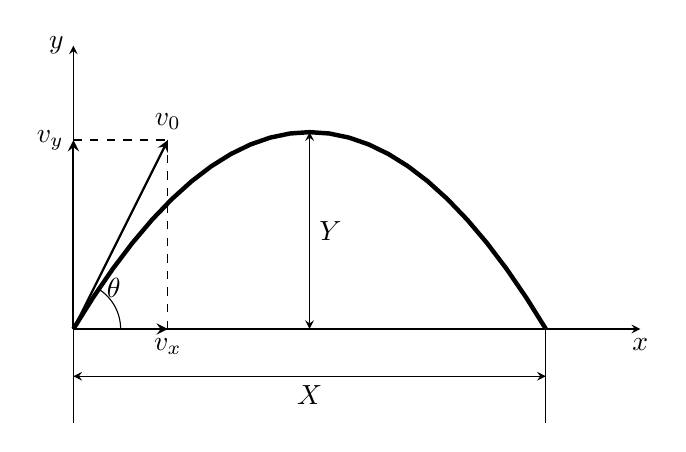
\begin{tikzpicture}[>=stealth, scale=1.2,domain=0:5]
  \draw[<->] (0,3)node [left]{$y$}--(0,0)--(6,0)node [below]{$x$};
  \draw[ultra thick] plot (\x,-0.3333*\x*\x+1.6667*\x ) ;
  \draw[<->] (0,-.5)--node [below]{$X$}(5,-.5);
  \draw (0,0)--(0,-1);
  \draw (5,0)--(5,-1);
  \draw[<->](2.5,0)--node [right]{$Y$}(2.5,6.25/3);
  \draw [->, thick](0,0)--(1,2)node [above]{$v_0$};
  \draw [dashed](1,0)node [below]{$v_x$}--(1,2);
  \draw [dashed](0,2)node [left]{$v_y$}--(1,2);
  \draw [thick,->](0,0)--(0,2);
  \draw [thick,->](0,0)--(1,0) ;
  \draw (.5,0) arc (0:60:.5) node [right]{$\theta$};
\end{tikzpicture}
\end{document}